% report.tex - generated
\documentclass[11pt,a4paper]{article}
\usepackage[utf8]{inputenc}
\usepackage{tikz}
\usepackage{geometry}
\geometry{margin=1in}
\title{Netzwerk- und Systembericht: Discovery \& Fix}
\author{Automatisch generiert}
\date{2026-01-17}

\begin{document}
\maketitle
\section{Kurzfassung}
Dieser Bericht dokumentiert Ursache und Behebung des UDP-Discovery-Problems.

\section{Systemaufbau (vor dem Fix)}
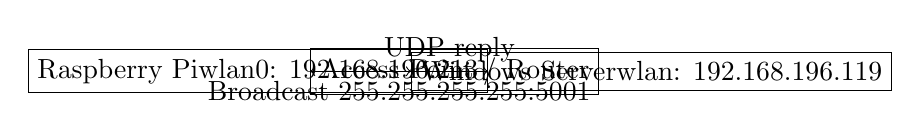
\begin{tikzpicture}[node distance=2.5cm,auto]
\node[draw,rectangle] (pi) {Raspberry Pi\\wlan0: 192.168.196.213};
\node[draw,rectangle,right of=pi] (ap) {Access Point / Router};
\node[draw,rectangle,right of=ap] (win) {Windows Server\\wlan: 192.168.196.119};
\draw[->] (pi) -- node {Broadcast 255.255.255.255:5001} (ap);
\draw[->] (ap) -- (win);
\draw[->,dashed] (win) -- node {UDP reply} (pi);
\end{tikzpicture}

\section{Ursache}
Broadcasts wurden im neuen Schulnetz teilweise gefiltert oder nicht an die Server-Schnittstelle weitergereicht; daher kamen keine Reply-Pakete an.

\section{Fix}
Der Server sendet nun die IP-Adresse seiner Schnittstelle, die zum anfragenden Client erreichbar ist. Der Client sollte zusätzlich gerichtete Broadcasts und Unicast-Probes verwenden.

\section{Warum der Fix funktioniert}
Weil der Client anhand der gelieferten, direkt erreichbaren IP eine funktionierende HTTP-URL bauen kann.

\section{Netzwerk-Checks}
Siehe `docs/network_report.md` f"ur tcpdump- und pktmon-Befehle.

\end{document}
